\documentclass[a4paper,finnish]{article}

\usepackage[finnish]{babel}
\usepackage[utf8]{inputenc}
\usepackage[sfdefault]{noto}
\usepackage[T1]{fontenc}
\usepackage{graphicx}
\usepackage{fullpage}
\usepackage{float}


% testing
\usepackage{blindtext}
\usepackage{color}
\usepackage{soulutf8}

\graphicspath{{../kuvat/}}
\usepackage[style=authoryear, maxcitenames=2]{biblatex}
\bibliography{sulautettujen-tuotteistaminen}


\newcommand{\TODO}[1]{\noindent{\hl{\textbf{TODO:}\quad#1}}}

\author{Jonas Nikula, 240497}
\title{Vahvistusoppimisen sovellukset langattomissa anturiverkoissa ja sen
vaikutukset tuotekehityksessä}
\date{\today}

\begin{document}
\maketitle

\begin{abstract}

  Anturiverkot ovat kasvava ilmiö, joilla on useita sovelluskohteita.
  Edullisten ja pienten verkotettujen antureiden seurauksena on entistä
  helpompaa kerätä paljon dataa laajoiltakin alueilta. Modernit anturiverkot
  saattavat koostua staattisten mikroantureiden lisäksi myös liikkuvista
  droneista.  Antureiden keräämän datan määrä ja niiden vaikeat
  toimintaolosuhteet luovat haasteita verkkojen tiedonsiirrolle. Näiden
  haasteiden ratkaisuun tarvitaan älykkäitä ratkaisuja, joista yksi on
  vahvistusoppimisen hyödyntäminen reitityksessä.  Vahvistusoppiminen on
  koneoppimisen alalaji jossa toimijalle pyritään opettamaan paras toimintatapa
  toimintaympäristössään. Vahvistusoppimista hyödyntävät anturiverkot pystyvät
  sopeutumaan muuttuviin ja vaikeisiin olosuhteisiin ja reitittämään dataa
  tehokkaasti ja luotettavasti.


  \subsubsection*{Avainsanat}
  Internet of Things, langattomat verkot, langattomat
  anturiverkot, koneoppiminen, vahvistusoppiminen
\end{abstract}


% include/input sections here
\section{Johdanto}
Langattomat anturiverkot ovat IOT:n kehityksen myötä yleistyneet monilla
aloilla. Anturien ja niiden keräämän datan lisääntyminen on luonut haasteita
verkkojen tehokkaalle toiminnalle. Tämän lisäksi niiden liikkuvuus erilaisten
alustojen ja robottien mukana on liisääntymässä, joka tuo omat haasteensa
niiden kehitykselle.

Tässä työssä käsitellään vahvistusoppimisen sovelluksia anturiverkkojen
verkkoliikenteen optimoinnille, ja kuinka se vaikuttaa tuotekehitykseen. Työ
perustuu pitkälti lähteiden~\cite{Arya2015} ja~\cite{Yu2006} tuloksiin.

\section{Käsitteiden määrittely}

\begin{description}

  \item [Internet of things, IoT] Suomennettuna ``esineiden internet'', usein
    käytetään lyhennettä IoT. IoT on laaja konsepti, ja tieteen ja teollisuuden
    kirjallisuudessa on jonkun verran epäselvyyttä siitä mitä termi pitää
    sisällään. IoT:ssa on kumminkin keskeistä erilaisten esineiden (things)
    verkottaminen toisten esineiden ja laajemman internetin kanssa. Keskeistä
    on myös että nämä esineet toimivat yhteistyössä keräämällä, käsittelemällä
    ja toimimalla datan perusteella.~\cite{Atzori2010a, Gubbi2013}

  \item [Anturiverkot] koostuvat toisiinsa linkitetyistä antureista. Nykyään
    puhutaan käytännössä langattomista verkoista (Wireless Sensor Network,
    WSN).  Anturit voivat pysyä paikallaan tai olla liikkuvia, esimerkiksi
    robotteja tai droneja. Antureiden keräämä data voidaan käsitellä joko
    keskitetysti, tai sitten hajautetusti.~\cite{Chong2003, Tubaishat2003}

  \item [Koneoppiminen] (machine learning) Tarkoittaa erilaisten mallien
    luomista datan perusteella. Käytetään tilanteissa joissa ihminen ei kykene
    luomaan matemaattista mallia, johtuen yleensä datan määrästä ja
    monimuotoisuudesta.  Termi käsittää useampia alatermejä jotka voivat olla
    hyvinkin erilaisia.~\cite{Grosan2011}

  \item [Vahvistusoppiminen] (reinforcement learning) on koneoppimisen alalaji,
    josta käytetään myös nimitystä ``robottioppiminen'', koska se on sen
    yleisin sovelluskohde.  Vahvistusoppimisessa koneoppimismallia muokataan
    ympäristön ja tilanteen mukaan. Vahvistusoppiminen perustuu oppijan
    (robotti, tekoäly tms) palkitsemiseen tai rankaisemiseen riippuen siitä
    kuinka hyvin se suorittaa sille annetun tehtävän (reitin etsiminen, pelin
    pelaaminen tms). Palkkion ja rankaisun tulisi vaikuttaa oppijan toimintaan
    niin että sen suoriutuminen tehtävästä paranee.~\cite{Kaelbling1996}

\end{description}

\section{Modernien anturiverkkojen tiedonsiirto-ongelmat}
\label{sec:problem}

Anturiverkkojen toimintaolosuhteista johtuen verkon yhteydet ovat muuttuvia ja
ennalta-arvaamattomia. Usein verkon yksittäisillä antureilla ei ole tietoa
verkon koostumuksesta sen välittömien naapureiden lisäksi. Siksi
reititysprotokollien täytyy pystyä sopeutumaan muuttuviin tilanteisiin
mahdollisimman vähällä informaatiolla itse verkosta.

Ensimmäinen artikkeli keskittyy anturiverkkojen keräämän datan tehokkaaseen
yhdistämiseen (engl.\ data fusion). Toinen taas pyrkii kehittämään
reititysprotokollan joka on robusti ja pystyy mukautumaan antureiden
tuhoutumisesta johtuviin muutoksiin.

\subsection{Datan yhdistäminen}
Artikkelissa~\cite{Yu2006} keskeistä on anturien keräämän datan yhdistäminen.
Datan yhdistäminen tarkoittaa että toisiinsa liittyvä data kerätään yhteen
kokonaiskuvan saamiseksi. Artikkeli
käyttää esimerkkinä UAV:sta koostuvaa anturiverkkoa, joissa jokaisella
yksittäisellä UAV:lla on matala varmuus kokonaistilanteesta. Datan yhdistäminen on
tärkeää jotta verkolla on vahva käsitys tilanteesta jonka avulla se voi
suunnitella toimintaansa.

Datan yhdistäminen toimii niin että toisiinsa liittyvä data koitetaan kerätä yhteen.
Verkon solmut lähettävät dataa eteenpäin kunnes jollakin solmulla on tarpeeksi
paljon dataa, jolloin se lopettaa datan eteenpäinlähetyksen ja rupeaa
prosessoimaan dataa ja tekemään sen avulla päätöksiä.

\subsection{Luotettava tiedonsiirto anturiverkoissa}
Anturiverkon solmujen kuolemat ovat ongelma jonka verkon täytyy pystyä
kestämään ja käsittelemään. Kuolema tarkoittaa tässä kontekstissa mitä tahansa
tilannetta jossa solmu on toimintakyvytön tai sen toimintakyky on niin huono
että siitä ei ole hyötyä verkossa. Artikkelissa~\cite{Arya2015} esitelty
algoritmi pyrkii etsimään solmujen kuolemista syntyviä reikiä ja
reitittämään data optimaalisesti ne huomioon ottaen.

% \TODO{Ehkä yksi kappale lisää tähän? Tai jos ei niin sitten yhdistä toiseen
% sektioon}

% \subsection{Muita anturiverkkojen reititysalgoritmeja}
% \TODO{Kerro joistain muista reititysprotokollista, ja siitä miksi ne eivät
% sovellu kuitenkaan tässä esitettyihin ongelmiin}

\section{Vahvistumisoppiminen anturiverkojen tiedonsiirrossa}
\label{sec:solution}

Kummatkin artikkelit siis ryhtyvät ratkaisemaan anturiverkkojen tiedonsiirron
reitityksen optimointia. Molemmat myös pyrkivät löytämään nopeita ja
luotettavia yhteyksiä solmujen väleille. Ensimmäinen kuitenkin pyrkii
pääasiassa etsimään verkon reikiä ja toinen pyrkii optimoimaan datan
yhdistämistä.

Vahvistusoppimisessa voidaan ajatella olevan kolme komponenttia
\begin{description}
  \item[Toimija (engl.\ agent)] on vahvistusoppimisen opetuksen kohde. Esimerkiksi
    robotti, jonka tulee oppia nopein reitti päämääräänsä.
  \item[Toiminta (engl.\ action)] on jotain mitä toimija voi tehdä. Esimerkiksi ``liiku
    pohjoisessa olevaan huoneeseen''.
  \item[Ympäristö (engl.\ environment)] vaikuttaa toimijan mahdollisiin toimintoihin ja
    niiden onnistumiseen. Toimintojen hyöty voi olla erittäin riippuvainen
    toimintaympäristöstä. Edelliseen esimerkkiin liittyen liikkuminen
    pohjoiseen ei välttämättä ole aina paras toiminto. Pohjoiseen vievä reitti
    voi olla esimerkiksi umpikuja.
\end{description}
Kuten kappaleessa~\ref{sec:terms} jo sanottiin, vahvistusoppimisessa oppijan,
eli toimijan, tulee löytää ympäristössään optimaalinen toiminta. Se löytää, tai
oppii tämän optimaalisen toiminnan kokeilemalla eri toimintoja. Tehdessään
toiminnon, se saa siitä jollain tavalla palautetta, joka vaikuttaa siihen minkä
toiminnon se valitsee ensi kerralla; Jos palaute oli positiivista, se valitsee
saman toiminnon. Jos taas negatiivista, se luultavasti kokeilee muuta
toimintoa.

Q-oppiminen (engl.\ Q-learning) on yksi vahvistusoppimisen menetelmä. Menetelmä
ei vaadi tarkkaa mallia ympäristöstä, ja siten soveltuu lähes mihin tahansa
vahvistusoppimisongelmaan.  Q-oppimisessa toimijan potentiaalisilla
toiminnoilla toimitaympäristössään on joku hyöty, eli Q-arvo. Kriittistä
Q-oppimisessa on Q-arvon päivittäminen toiminnasta saadun palautteen avulla;
Tämä on menetelmän tapa oppia optimaalinen toimintatapa ympäristössä.
Q-oppiminen pyrkii ottamaan huomioon myös ajan. Ajan huomioiminen on tärkeää
koska varsinkin reaalimaailmassa useimmat toiminnot eivät ole heti palkitsevia,
vaan ne mahdollistavat tulevaisuudessa toimintoja jotka ovat arvokkaita.
Toiminnan lopullinen hinta määräytyy siis nykyisen tilan lisäksi tiloista
joihin toiminto johtaa.~\parencite{Kaelbling1996}

\subsection{Datan tehokas yhdistäminen vahvistusoppimisen avulla}

Yksinkertainen algoritmi datan yhdistämiseen anturiverkossa on polunvahvistusalgoritmi
(engl.\ path reinforcement).
Kun algoritmi ensimmäisen kerran saa dataa tietystä
tapahtumasta, se lähettää sen satunnaiselle naapurille eteenpäin. Kun se saa
samasta tapahtumasta lisää dataa, se lähettää sen eteenpäin sille naapurille
jolle se viimeksi lähetti dataa kyseisestä tapahtumasta.  Kuvassa~\ref{fig:yu2006} on
havainnollistettu sitä kuinka polunvahvistusalgoritmi pyrkii lähettämään
toisiinsa liittyvän datan samalle solmulle. Tapahtuman ja datan
samankaltaisuuden tai liittyvyyden määrittely on oma ongelmansa johon
artikkelissa~\cite{Yu2006} ei oteta kantaa. Algoritmin ideana on että jos data
reititetään aina samaa reittiä pitkin, todennäköisyys että jollekin reitin
solmulle tulee tarpeeksi dataa kasvaa.

\begin{figure}[h]
  \centering
  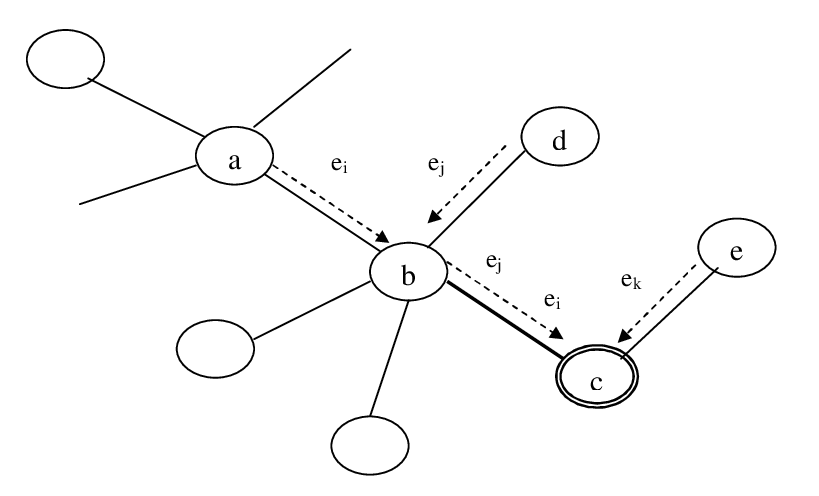
\includegraphics[width=0.8\linewidth]{yu2006_kuva}
  \caption{Polunvahvistusalgoritmin havainnekuva.~\parencite{Yu2006}}
\label{fig:yu2006}
\end{figure}

Vaikka kyseinen algoritmi edistää datan yhdistämistä melko tehokkaasti ilman kattavaa
tietoa anturiverkosta, sen ongelmana on että se ei ota huomioon verkon
yhteyksien laatua, tai edes sitä meneekö tieto perille. Eli se pyrkii
lähettämään dataa samalle naapurille vaikka yhteys olisi huono tai jopa
olematon. Ongelma voidaan korjata lähettämällä data uudestaan jos vikoja tai
huonoja yhteyksia havaitaan verkossa. Uudelleenlähetys kuitenkin laskee
algoritmin tehokkuutta melko paljon, koska uuden naapurin valinta on
satunnaista jolloin data saatetaan lähettää uudestaan vialliselle naapurille,
tai muuten epäoptimaaliselle naapurille.

Tehokkuutta voidaan parantaa mallintamalla naapureiden luotettavuutta jollain
tavalla. Tässä päästäänkin artikkelin~\cite{Yu2006} keskeiseen algoritmiin,
jota tekijät itse kutsuvat polunoppimisalgoritmiksi (engl.\ path learning).
Perusidea datan yhdistämisen kannalta on sama kuin polunvahvistuksessakin;
Samankaltainen data pyritään reitittämään samaa reittiä pitkin, jotta
todennäköisyys että data päätyy samalle solmulle on korkeampi. Algoritmi
käyttää kuitenkin vahvistusoppimista hyväkseen opettemalla solmuille toiminnan
myötä mitkä naapurit pystyvät luotettavimmin lähettämään dataa myös eteenpäin.

Artikkelissa~\cite{Yu2006} tehtyjen simuulatioiden perusteella kyseinen
algoritmi parhaimmillaan kaksinkertaistaa datan yhdistymisen todennäköisyyden
verrattuna satunnaiskävely (engl.\ random walks) algoritmiin, jossa
vastaanottaja siis valitaan satunnaisesti. Algoritmi kestää myös hyvin solmujen
tuhoutumista; Tilanteessa jossa jopa 50\% solmuista tuhoutui, datan
yhdistymisen todennäköisyys oli 70\%.

\subsection{Vahvistusoppimisen hyödyntäminen sopeutuvassa anturiverkossa}

Kuten datan yhdistämisessä, myös artikkelissa~\cite{Arya2015} käytetään hyväksi
vahvistusoppimista tehokkaan reititysprotokollan luomiseksi. Kuten datan
yhdistämiseen
keskittyvän algoritmin kanssa, sopeutuvan reitityksen algoritmi pyrkii
huomioimaan solmun naapureiden luotettavuutta. Kyseinen algoritmi ottaa
kuitenkin myös huomioon muita muuttujia, kuten vastaanottajan akkutilanteen.
Lisäksi tässä algoritmissa otetaan huomioon koko reitti päämäärään asti, ei
ainoastaan hyppy naapurille. Myös tässä algoritmissa vastaanottajan hyvyys
määräytyy sen antaman palautteen mukaan. Yhden solmun oppiminen voidaan siis
kuvata tapahtumaketjuna, jossa se
\begin{enumerate}
  \item Valitsee naapureistaan vastaanottajan niiden Q-arvon perusteella
  \item Lähettää datan eteenpäin valitulle naapurille
  \item Päivittää naapurin Q-arvon siltä saadun palautteen perusteella
\end{enumerate}
Kuvassa~\ref{fig:arya2015_oppiminen} on yksinkertainen
systeemikuva~\cite{Arya2015} kuvaaman vahvitusoppimista käyttävän algoritmin
toiminnasta.

Luotettavan reitityksen lisäksi kyseisen algoritmin keskeisiä päämääriä on
tunnistaa reiät anturiverkon kattavuudessa. Reiät kattavuudessa syntyvät kun
antureita vioittuu tai ne eivät jostain muusta syystä pysty keräämään tai
reitittämään dataa tarpeeksi hyvin. Tämän seurauksena verkkoon muodostuu
reikä, jonka läpi ei voi lähettää dataa, vaan tiedonsiirron täytyy mukautua
sen ympärille. Reiän havaitseminen on siis tärkeää optimaalisen reitityksen
kannalta. Useimmissa anturiverkon sovelluksissa on myös erittäin hyödyllistä
olla tietoinen miltä alueilta ei saada tietoa; Myös tämän takia on tärkeää
havaita verkon reiät.

Jotta reikiä voidaan löytää täytyy ensin etsiä optimaalinen reititys olemassa
olevalle verkolle. Tämä tapahtuu edellä kuvatulla tavalla. Aluksi verkon nielut
myös pyytävät antureita ja muita solmuja lähettämään itsestään dataa verkon
yli, jotta optimaalinen reititys löytyisi mahdollisimman nopeasti; Verkon
reitityshän perustuu vahvistusoppimiseen, joten optimaalista reittiä ei saada
selville ilman että tiedonsiirtoa kokeillaan. Kun optimaalinen reititys on
löydetty, voidaan ruveta havaitsemaan reikiä. Jos solmu itse havaitsee
vioittuneensa se pyrkii lähettämään viestin tilastaan. Tämän viestin avulla sen
naapurit voivat päivittää omat tietonsa kyseisestä solmusta. Tämän lisäksi
tukiasema ajaa säännöllisesti algoritmia jonka on tarkoitus havaita reiät
joista solmut itse eivät ole ilmoittaneet.

\begin{figure}[h]
  \centering
  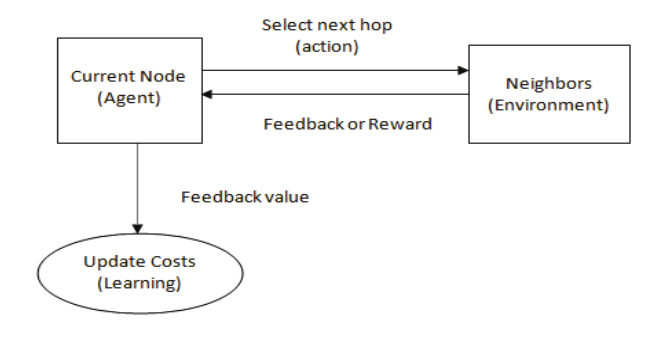
\includegraphics[width=0.8\linewidth]{arya2015_oppiminen}
  \caption{Systeemikuva reititysalgoritmin vahvistusoppimisesta.~\parencite{Arya2015}}
\label{fig:arya2015_oppiminen}
\end{figure}

Artikkelissa on myös simuloitu algoritmin toimintaa ja suorituskykyä.
Kuvassa~\ref{fig:arya2015} näkyy simuloitu tilanne, jossa osa solmuista on
tuhoutunut. Tuhoutuneiden solmujen seurauksena syntynyt reikä näkyy mustana.

\begin{figure}[h]
  \centering
  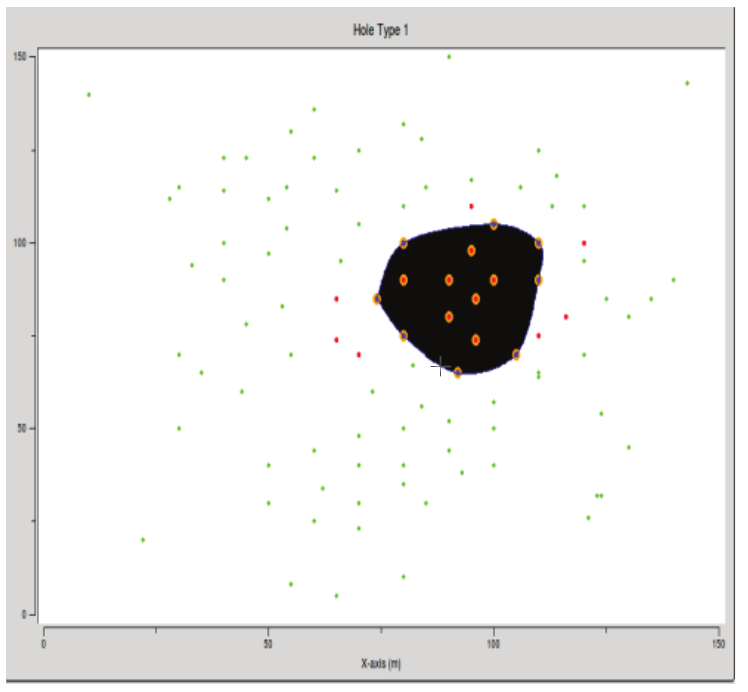
\includegraphics[width=0.8\linewidth]{arya2015_kuva}
  \caption{Simulaatiokuva artikkelista~\cite{Arya2015}.}
\label{fig:arya2015}
\end{figure}


\section{Johtopäätökset}
Tämän kirjallisuusselvityksen pohjalta voidaan todeta että vahvistusoppimisella
on potentiaalia anturiverkkojen reitityksessä. Anturiverkkojen
toimintaolosuhteet vaativat reititysalgoritmeiltä mukautuvuutta ja tehokkuutta.
Näihin vaatimuksiin voidaan vastata vahvistusoppimisen menetelmillä.


\clearpage{}
\printbibliography{}

\end{document}
